\documentclass[conference]{IEEEtran}
%% SECON 2013 addition:
\makeatletter
\def\ps@headings{%
\def\@oddhead{\mbox{}\scriptsize\rightmark \hfil \thepage}%
\def\@evenhead{\scriptsize\thepage \hfil \leftmark\mbox{}}%
\def\@oddfoot{}%
\def\@evenfoot{}}
\makeatother
\pagestyle{headings} 

\ifCLASSINFOpdf
  % \usepackage[pdftex]{graphicx}
  % declare the path(s) where your graphic files are
  % \graphicspath{{../pdf/}{../jpeg/}}
  % and their extensions so you won't have to specify these with
  % every instance of \includegraphics
  % \DeclareGraphicsExtensions{.pdf,.jpeg,.png}
\else
  % or other class option (dvipsone, dvipdf, if not using dvips). graphicx
  % will default to the driver specified in the system graphics.cfg if no
  % driver is specified.
  % \usepackage[dvips]{graphicx}
  % declare the path(s) where your graphic files are
  % \graphicspath{{../eps/}}
  % and their extensions so you won't have to specify these with
  % every instance of \includegraphics
  % \DeclareGraphicsExtensions{.eps}
\fi
% *** MATH PACKAGES ***
%
\usepackage[cmex10]{amsmath}
\usepackage{amsfonts}
\usepackage{graphicx, epsfig}
\usepackage{color}
\usepackage{subfigure}
\usepackage{xspace}
\usepackage{algorithm}
\usepackage{algpseudocode}
\usepackage{breqn}
\usepackage{cite}

\renewcommand{\thealgorithm}{}
\algnewcommand{\LineComment}[1]{\State \(\triangleright\) #1}
% A popular package from the American Mathematical Society that provides
% many useful and powerful commands for dealing with mathematics. If using
% it, be sure to load this package with the cmex10 option to ensure that
% only type 1 fonts will utilized at all point sizes. Without this option,
% it is possible that some math symbols, particularly those within
% footnotes, will be rendered in bitmap form which will result in a
% document that can not be IEEE Xplore compliant!
%
%\usepackage{array}
%\usepackage{mdwmath}
%\usepackage{mdwtab}
%\usepackage{eqparbox}
%\usepackage[tight,footnotesize]{subfigure}
%\usepackage[caption=false]{caption}
%\usepackage[font=footnotesize]{subfig}
%\usepackage[caption=false,font=footnotesize]{subfig}
%
%\usepackage{fixltx2e}

%\usepackage{stfloats}

%\usepackage{url}

% correct bad hyphenation here
\hyphenation{net-works}

\DeclareMathOperator*{\E}{\mathbb{E}}

\begin{document}
%
% paper title
% can use linebreaks \\ within to get better formatting as desired
\title{Modeling Memory and Information Flow in a Human Network}

\IEEEoverridecommandlockouts

% author names and affiliations
% use a multiple column layout for up to three different
% affiliations

%\author{\IEEEauthorblockN{Scott Rager}
%\IEEEauthorblockA{Department of Computer Science and Engineering\\
%Pennsylvania State University\\
%University Park, PA 16802\\
%Email: rager@psu.edu}}

%\author{\IEEEauthorblockN{Scott Rager, Ertugrul Ciftcioglu, Thomas La Porta}
%\IEEEauthorblockA{Department of Computer Science\\
%and Engineering\\
%Pennsylvania State University\\
%University Park, PA 16802\\
%Email: rager@psu.edu, enc118@psu.edu, tlp@cse.psu.edu}
%\and
%\IEEEauthorblockN{Alice Leung, William Dron}
%\IEEEauthorblockA{Raytheon BBN Technologies\\
%Cambridge, MA 02138\\
%Email: aleung@bbn.com, wdron@bbn.com}
%\and
%\IEEEauthorblockN{John Hancock}
%\IEEEauthorblockA{Artistech\\
%City, State Zip Code\\
%Email: johnh@artistech.com}
%}

%\author{
%  \IEEEauthorblockN{Scott T. Rager\IEEEauthorrefmark{1} \quad Ertugrul N. Ciftcioglu\IEEEauthorrefmark{2}  \quad Ram Ramanathan\IEEEauthorrefmark{3} \quad Thomas F. La Porta\IEEEauthorrefmark{1} \quad Ramesh Govindan\IEEEauthorrefmark{4} \\
%  }
%  \IEEEauthorblockA{
%  	\IEEEauthorrefmark{1}The Pennsylvania State University, University Park, PA 16802\\
%	\IEEEauthorrefmark{2}IBM Research, Yorktown Heights, NY 10598 \\
%  \IEEEauthorrefmark{3}Raytheon BBN Technologies, Cambridge, MA 02138 \\
%  \IEEEauthorrefmark{4}University of Southern California, Los Angeles, CA 90089
%  }
%
%  Email:  rager@psu.edu, enciftci@us.ibm.com , ramanath@bbn.com, tlp@cse.psu.edu, ramesh@usc.edu
%\thanks{Research was sponsored by the U.S. Army Research Laboratory under the Network Science Collaborative Technology Alliance, Agreement Number W911NF-09-2-0053.} 
%}


% for over three affiliations, or if they all won't fit within the width
% of the page, use this alternative format:
% 
%\author{\IEEEauthorblockN{Michael Shell\IEEEauthorrefmark{1},
%Homer Simpson\IEEEauthorrefmark{2},
%James Kirk\IEEEauthorrefmark{3}, 
%Montgomery Scott\IEEEauthorrefmark{3} and
%Eldon Tyrell\IEEEauthorrefmark{4}}
%\IEEEauthorblockA{\IEEEauthorrefmark{1}School of Electrical and Computer Engineering\\
%Georgia Institute of Technology,
%Atlanta, Georgia 30332--0250\\ Email: see http://www.michaelshell.org/contact.html}
%\IEEEauthorblockA{\IEEEauthorrefmark{2}Twentieth Century Fox, Springfield, USA\\
%Email: homer@thesimpsons.com}
%\IEEEauthorblockA{\IEEEauthorrefmark{3}Starfleet Academy, San Francisco, California 96678-2391\\
%Telephone: (800) 555--1212, Fax: (888) 555--1212}
%\IEEEauthorblockA{\IEEEauthorrefmark{4}Tyrell Inc., 123 Replicant Street, Los Angeles, California 90210--4321}}




% use for special paper notices
%\IEEEspecialpapernotice{(Invited Paper)}




% make the title area
\maketitle


%\begin{abstract}
%\boldmath
%%area
%%problem
%%solution
%%methodology
%%results
%%takeaway
%This is where the abstract will be....essentially we're looking at how information storage and QoI are different in computers vs. humans.
%
%\end{abstract}

% IEEEtran.cls defaults to using nonbold math in the Abstract.
% This preserves the distinction between vectors and scalars. However,
% if the conference you are submitting to favors bold math in the abstract,
% then you can use LaTeX's standard command \boldmath at the very start
% of the abstract to achieve this. Many IEEE journals/conferences frown on
% math in the abstract anyway.

% no keywords




% For peer review papers, you can put extra information on the cover
% page as needed:
% \ifCLASSOPTIONpeerreview
% \begin{center} \bfseries EDICS Category: 3-BBND \end{center}
% \fi
%
% For peerreview papers, this IEEEtran command inserts a page break and
% creates the second title. It will be ignored for other modes.
\IEEEpeerreviewmaketitle


\section{Introduction}
\label{sec:intro}

%area
We would like to look at QoI in individual nodes in a network and how it is modified by various factors.  Using this information, we can more effectively model QoI-aware networks.  Then, we also want to explore how these things apply when we look at social networks and/or include humans in the loop of information flow.
%problem

%why not solved

%insight
%contribution


%
\section{Related Work}
\label{sec:related_work}

Coming soon...


\section{Information Model}
\label{sec:info_model}

There are a number of agents that get factoids distributed to them.  Each of these factoids has about 1-3 pieces of information that can contribute to a solution, which itself is made up of 4 parts- who, what, where, and when.  Each contributes to the QoI by contributing to one or more parts of this solution.  For example, a factoid could be like "The Lion was seen in Psiland," which contributes to both the who and the where.  All of the agents are working toward their own solution, using the factoids they receive while also sharing them with their neighbor agents.  

For simplicity in evaluation, we can reduce the problem to a small number of categories, even just one, like who, for example.  We can also make some simplifications of the QoI contribution of each factoid to the solution part(s).  We can make a requirement that some number X of factoids need to be collected to get to the correct solution.  Then, we can expand it to a probabilistic problem in which the parts of each factoid add to a confidence probability in a particular solution.

We will assume a scenario in which $N$ pieces of intelligence, called factoids, are supplied to an agent.  Each of the $N$ factoids are uniquely identified by $i = \{1,..., N\}$, representing the order in which they are introduced to the agent.  We will represent the agent's ability to recall factoid $i$ with the random variable $R_i$ where $P(R_i = 1) = p_{r_i}$ and $0$ otherwise.  The value $p_{r_i}$ will be explained in Section \ref{sec:ser_pos_effect}.  

%\begin{eqnarray*}
%  f_{R_i} &=&
%    \left\{\begin{array}{ll}
%    p_{r_i} & \mbox{    } r_i = 1 \\
%    1-p_{r_i} & \mbox{    } r_i = 0 
%    \end{array}\right.
%\end{eqnarray*}

\section{Human Memory Model}
\label{sec:memory_model}

Dual-process theory of memory proposes that the brain stores both \emph{verbatim} and \emph{gist} representations of an event.  Since we will be focusing on intelligence factoids that contain specific details about a situation, which may also be obtained from another person and not from directly witnessing an event firsthand, we will exclusively consider the recall of verbatim traces.  

While a large number of factors can impact the encoding, storage, and recall of memories, we choose in this work to focus on only three well-studied components:  working memory capacity, the serial position effect, and bias encoding.  We address each of these factors' effects on the ability of recalling intelligence factoids.

\subsection{Working Memory Capacity}

The capacity of a persons' working memory is dependent on a few factors, such as the specific individual and the type of information being stored.  The variance in these differences of various memory capacities, however, is relatively small.  We can define the capacity of individual $x$ in a specific scenario as $K_x$ elements, where $K_x$ is a normal random variable given by $K_x = N( \mu_K, \sigma_K )$, where $\mu_k = U(\mu_{K_{min}},\mu_{K_{max}})$ is given by a uniform random variable with a defined minimum and maximum value and $\sigma_K$ is a given constant taken from empirical evaluations.  Using this model, different individuals' average capacities can be captured as well as the randomness of the capacity at various times or situations.

Since $K_x$ represents the likelihood of recalling each factoid, $i$ will partially depend on how many total factoids are presented.  Specifically, 

Question: Should the expected number of recall items should equal the capacity?:
\begin{equation}
	E [ \sum\limits_{i=1}^N R_{i}^x ] = K_x
\end{equation}
%If so, should that hold for all $N$?  For example, if my working memory capacity is $\approx 10$, do I remember $10$ things on average when 

\subsection{Serial Position Effect}
\label{sec:ser_pos_effect}

\begin{figure}
\begin{centering}
    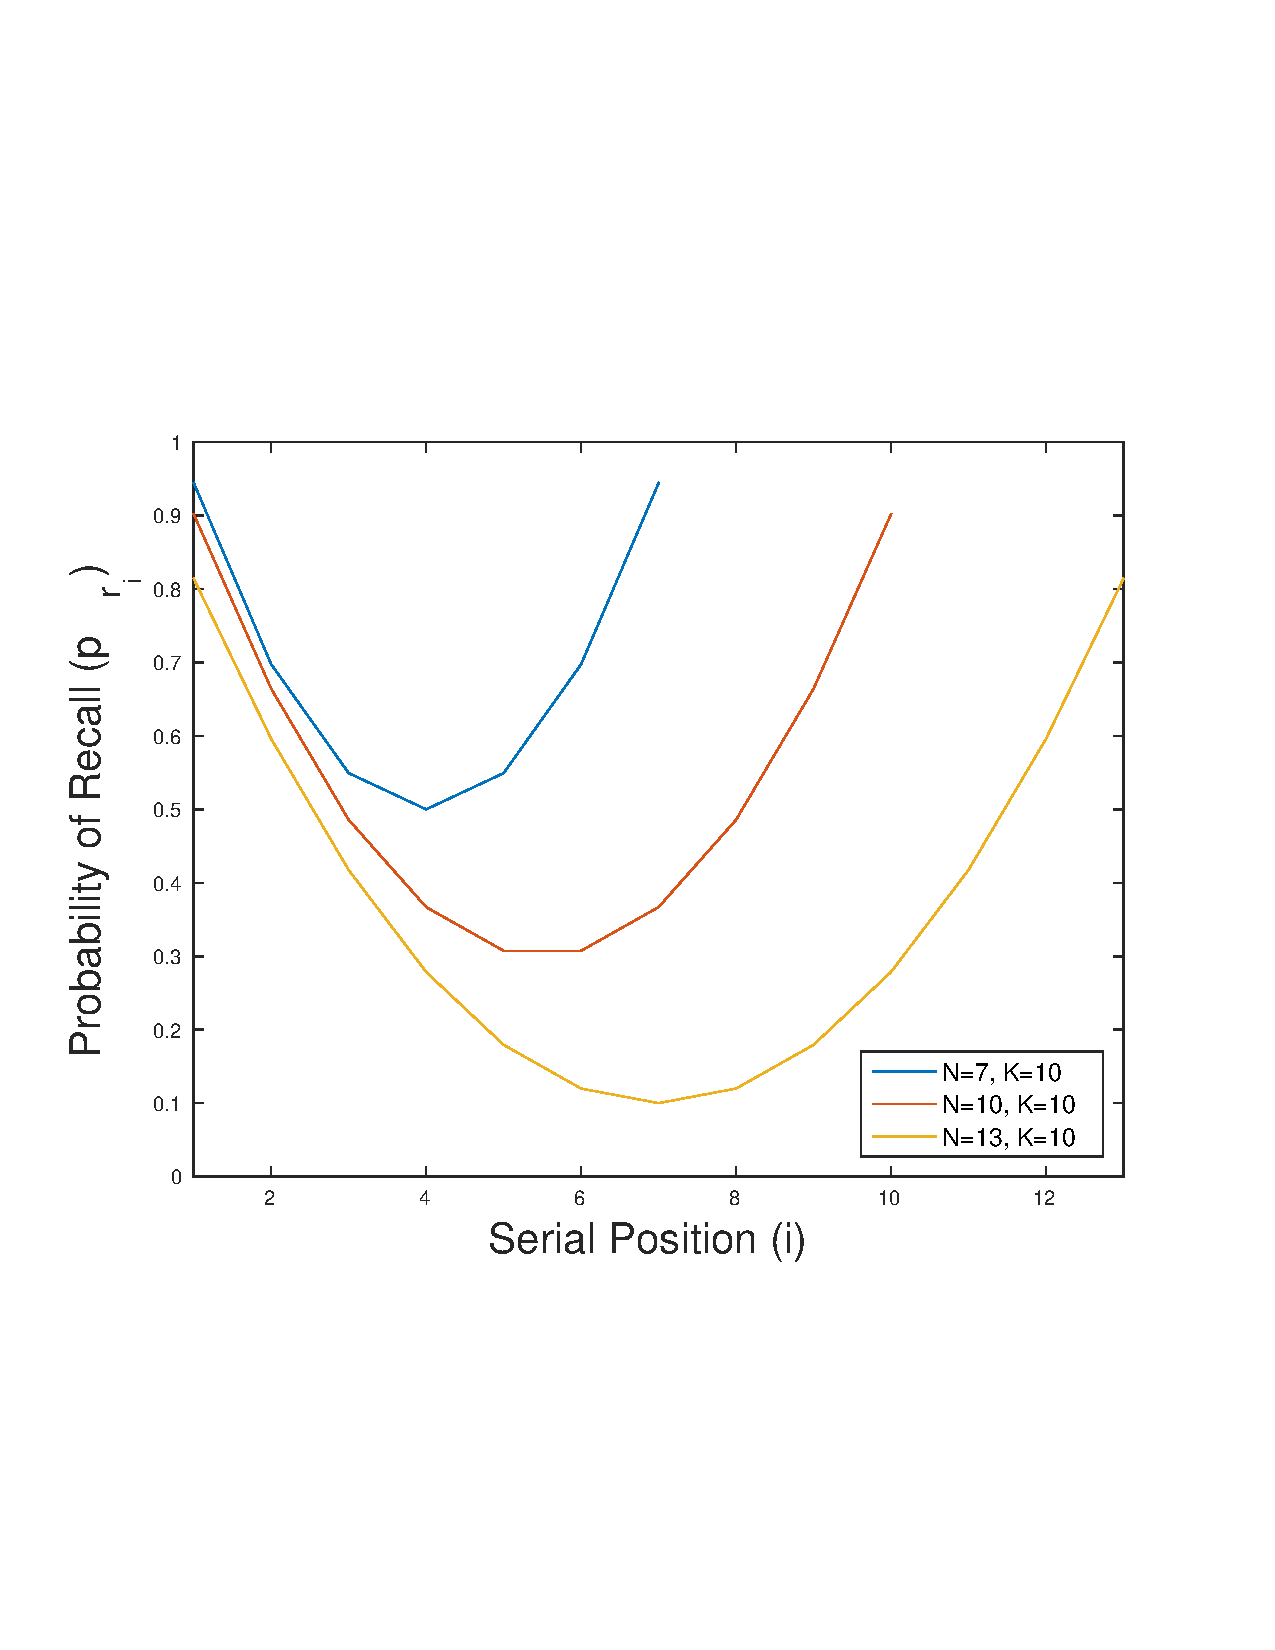
\includegraphics[clip=true, trim = 0mm 65mm 25mm 50mm, scale=0.50]{figures/mean_prob_recall_vs_ser_pos.pdf}
    \caption{ The mean probability of recall is impacted by the serial position effect and the amount of information relative to capacity. }
    \label{fig:prob_recall_vs_serial_pos}
\end{centering}
\end{figure}

The serial position effect describes the phenomenon by which people are more likely to recall the information presented to them first and last in a sequence than the information in the middle of the sequence.  Given $N$ and $K$, we can define a function for $p_{r_i} = f(N,K,i)$.  Figure \ref{fig:prob_recall_vs_serial_pos} shows examples of this function for an instance of $K=10$ and several example values of $N$ illuminating each possibility of $N < K$, $N = K$, and $N > K$.

Question:  The function used to generate the examples of $p_{r_i}$ is just a scaled parabola of the form:
\begin{equation}
    	f(N,K,i) = \frac{(i - \frac{N+1}{2})^2}{(\frac{N+1}{2} + p_{r_i-min})^2} + p_{r_i-min}
\end{equation}
where $\frac{N+1}{2}$ centers the function relative to $N$ and $p_{r_i-min}$ is a chosen value representing the minimum probability of recalling any item.
Are there any references that provide actual functions of the serial position effect data that we should use?  If not, meaning we do need to use a function that models it as best as we can, how close is this?  Should it be weighted more heavily on one side or the other, for example?

\subsection{Bias Encoding}

Question:  How can we incorporate this into the model?  

Proposal:  We can define subject areas $\mathcal{S} = \{S_1, ...S_M\}$.  An agent can be an expert (or familiar) with some subset of these subject areas, and each factoid can also be defined to belong to a subset of the subject areas.  Then we could introduce a scaling factor based on the overlap between an agent's area of expertise and how the factoid fits into it.  Is there any basis for this kind of thing in memory research?

\subsection{Note on $p_{r_i}$}
Here, I am defining $p_{r_i}$ to be a constant probability based on the values of $N$, $K$, and $i$.  An alternative that might make it more realistic, but possibly complicate analysis, would be to have it be a random variable itself.  It could be given by $N(\mu_{r_i}, \sigma_{r_i})$ where $\mu_{r_i}$ is given by a function of $N$, $K$, and $i$, just as $p_{r_i}$ is treated above.  



%
\section{Conclusion}
\label{sec:conclusion}

Coming soon...

% Problem
% Solution
% method and results
% Take away : Lesson
% Future work




%\appendix
%\input{sections/random_explanation}
% conference papers do not normally have an appendix


% use section* for acknowledgement
%\section*{Acknowledgment}


%The authors would like to thank...


% trigger a \newpage just before the given reference
% number - used to balance the columns on the last page
% adjust value as needed - may need to be readjusted if
% the document is modified later
%\IEEEtriggeratref{8}
% The "triggered" command can be changed if desired:
%\IEEEtriggercmd{\enlargethispage{-5in}}

% references section

% can use a bibliography generated by BibTeX as a .bbl file
% BibTeX documentation can be easily obtained at:
% http://www.ctan.org/tex-archive/biblio/bibtex/contrib/doc/
% The IEEEtran BibTeX style support page is at:
% http://www.michaelshell.org/tex/ieeetran/bibtex/
%\bibliographystyle{IEEEtran}
% argument is your BibTeX string definitions and bibliography database(s)
%\bibliography{IEEEabrv,../bib/paper}
%
% <OR> manually copy in the resultant .bbl file
% set second argument of \begin to the number of references
% (used to reserve space for the reference number labels box)
%\begin{thebibliography}{1}


\bibliographystyle{unsrt}

\bibliography{references}

%\bibitem{IEEEhowto:kopka}
%H.~Kopka and P.~W. Daly, \emph{A Guide to \LaTeX}, 3rd~ed.\hskip 1em plus
%  0.5em minus 0.4em\relax Harlow, England: Addison-Wesley, 1999.

%\end{thebibliography}




% that's all folks
\end{document}


